\documentclass[1p]{elsarticle_modified}
%\bibliographystyle{elsarticle-num}

%\usepackage[colorlinks]{hyperref}
%\usepackage{abbrmath_seonhwa} %\Abb, \Ascr, \Acal ,\Abf, \Afrak
\usepackage{amsfonts}
\usepackage{amssymb}
\usepackage{amsmath}
\usepackage{amsthm}
\usepackage{scalefnt}
\usepackage{amsbsy}
\usepackage{kotex}
\usepackage{caption}
\usepackage{subfig}
\usepackage{color}
\usepackage{graphicx}
\usepackage{xcolor} %% white, black, red, green, blue, cyan, magenta, yellow
\usepackage{float}
\usepackage{setspace}
\usepackage{hyperref}

\usepackage{tikz}
\usetikzlibrary{arrows}

\usepackage{multirow}
\usepackage{array} % fixed length table
\usepackage{hhline}

%%%%%%%%%%%%%%%%%%%%%
\makeatletter
\renewcommand*\env@matrix[1][\arraystretch]{%
	\edef\arraystretch{#1}%
	\hskip -\arraycolsep
	\let\@ifnextchar\new@ifnextchar
	\array{*\c@MaxMatrixCols c}}
\makeatother %https://tex.stackexchange.com/questions/14071/how-can-i-increase-the-line-spacing-in-a-matrix
%%%%%%%%%%%%%%%

\usepackage[normalem]{ulem}

\newcommand{\msout}[1]{\ifmmode\text{\sout{\ensuremath{#1}}}\else\sout{#1}\fi}
%SOURCE: \msout is \stkout macro in https://tex.stackexchange.com/questions/20609/strikeout-in-math-mode

\newcommand{\cancel}[1]{
	\ifmmode
	{\color{red}\msout{#1}}
	\else
	{\color{red}\sout{#1}}
	\fi
}

\newcommand{\add}[1]{
	{\color{blue}\uwave{#1}}
}

\newcommand{\replace}[2]{
	\ifmmode
	{\color{red}\msout{#1}}{\color{blue}\uwave{#2}}
	\else
	{\color{red}\sout{#1}}{\color{blue}\uwave{#2}}
	\fi
}

\newcommand{\Sol}{\mathcal{S}} %segment
\newcommand{\D}{D} %diagram
\newcommand{\A}{\mathcal{A}} %arc


%%%%%%%%%%%%%%%%%%%%%%%%%%%%%5 test

\def\sl{\operatorname{\textup{SL}}(2,\Cbb)}
\def\psl{\operatorname{\textup{PSL}}(2,\Cbb)}
\def\quan{\mkern 1mu \triangleright \mkern 1mu}

\theoremstyle{definition}
\newtheorem{thm}{Theorem}[section]
\newtheorem{prop}[thm]{Proposition}
\newtheorem{lem}[thm]{Lemma}
\newtheorem{ques}[thm]{Question}
\newtheorem{cor}[thm]{Corollary}
\newtheorem{defn}[thm]{Definition}
\newtheorem{exam}[thm]{Example}
\newtheorem{rmk}[thm]{Remark}
\newtheorem{alg}[thm]{Algorithm}

\newcommand{\I}{\sqrt{-1}}
\begin{document}

%\begin{frontmatter}
%
%\title{Boundary parabolic representations of knots up to 8 crossings}
%
%%% Group authors per affiliation:
%\author{Yunhi Cho} 
%\address{Department of Mathematics, University of Seoul, Seoul, Korea}
%\ead{yhcho@uos.ac.kr}
%
%
%\author{Seonhwa Kim} %\fnref{s_kim}}
%\address{Center for Geometry and Physics, Institute for Basic Science, Pohang, 37673, Korea}
%\ead{ryeona17@ibs.re.kr}
%
%\author{Hyuk Kim}
%\address{Department of Mathematical Sciences, Seoul National University, Seoul 08826, Korea}
%\ead{hyukkim@snu.ac.kr}
%
%\author{Seokbeom Yoon}
%\address{Department of Mathematical Sciences, Seoul National University, Seoul, 08826,  Korea}
%\ead{sbyoon15@snu.ac.kr}
%
%\begin{abstract}
%We find all boundary parabolic representation of knots up to 8 crossings.
%
%\end{abstract}
%\begin{keyword}
%    \MSC[2010] 57M25 
%\end{keyword}
%
%\end{frontmatter}

%\linenumbers
%\tableofcontents
%
\newcommand\colored[1]{\textcolor{white}{\rule[-0.35ex]{0.8em}{1.4ex}}\kern-0.8em\color{red} #1}%
%\newcommand\colored[1]{\textcolor{white}{ #1}\kern-2.17ex	\textcolor{white}{ #1}\kern-1.81ex	\textcolor{white}{ #1}\kern-2.15ex\color{red}#1	}

{\Large $\underline{12n_{0168}~(K12n_{0168})}$}

\setlength{\tabcolsep}{10pt}
\renewcommand{\arraystretch}{1.6}
\vspace{1cm}\begin{tabular}{m{100pt}>{\centering\arraybackslash}m{274pt}}
\multirow{5}{120pt}{
	\centering
	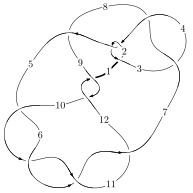
\includegraphics[width=112pt]{../../../GIT/diagram.site/Diagrams/png/2257_12n_0168.png}\\
\ \ \ A knot diagram\footnotemark}&
\allowdisplaybreaks
\textbf{Linearized knot diagam} \\
\cline{2-2}
 &
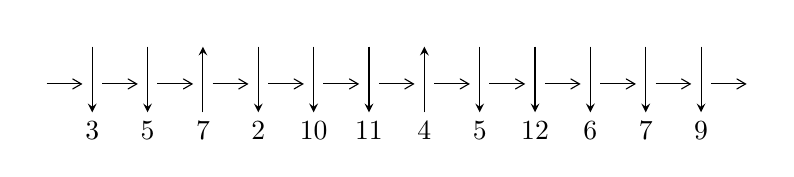
\begin{tikzpicture}[x=20pt, y=17pt]
	% nodes
	\node (C0) at (0, 0) {};
	\node (C1) at (1, 0) {};
	\node (C1U) at (1, +1) {};
	\node (C1D) at (1, -1) {3};

	\node (C2) at (2, 0) {};
	\node (C2U) at (2, +1) {};
	\node (C2D) at (2, -1) {5};

	\node (C3) at (3, 0) {};
	\node (C3U) at (3, +1) {};
	\node (C3D) at (3, -1) {7};

	\node (C4) at (4, 0) {};
	\node (C4U) at (4, +1) {};
	\node (C4D) at (4, -1) {2};

	\node (C5) at (5, 0) {};
	\node (C5U) at (5, +1) {};
	\node (C5D) at (5, -1) {10};

	\node (C6) at (6, 0) {};
	\node (C6U) at (6, +1) {};
	\node (C6D) at (6, -1) {11};

	\node (C7) at (7, 0) {};
	\node (C7U) at (7, +1) {};
	\node (C7D) at (7, -1) {4};

	\node (C8) at (8, 0) {};
	\node (C8U) at (8, +1) {};
	\node (C8D) at (8, -1) {5};

	\node (C9) at (9, 0) {};
	\node (C9U) at (9, +1) {};
	\node (C9D) at (9, -1) {12};

	\node (C10) at (10, 0) {};
	\node (C10U) at (10, +1) {};
	\node (C10D) at (10, -1) {6};

	\node (C11) at (11, 0) {};
	\node (C11U) at (11, +1) {};
	\node (C11D) at (11, -1) {7};

	\node (C12) at (12, 0) {};
	\node (C12U) at (12, +1) {};
	\node (C12D) at (12, -1) {9};
	\node (C13) at (13, 0) {};

	% arrows
	\draw[->,>={angle 60}]
	(C0) edge (C1) (C1) edge (C2) (C2) edge (C3) (C3) edge (C4) (C4) edge (C5) (C5) edge (C6) (C6) edge (C7) (C7) edge (C8) (C8) edge (C9) (C9) edge (C10) (C10) edge (C11) (C11) edge (C12) (C12) edge (C13) ;	\draw[->,>=stealth]
	(C1U) edge (C1D) (C2U) edge (C2D) (C3D) edge (C3U) (C4U) edge (C4D) (C5U) edge (C5D) (C6U) edge (C6D) (C7D) edge (C7U) (C8U) edge (C8D) (C9U) edge (C9D) (C10U) edge (C10D) (C11U) edge (C11D) (C12U) edge (C12D) ;
	\end{tikzpicture} \\
\hhline{~~} \\& 
\textbf{Solving Sequence} \\ \cline{2-2} 
 &
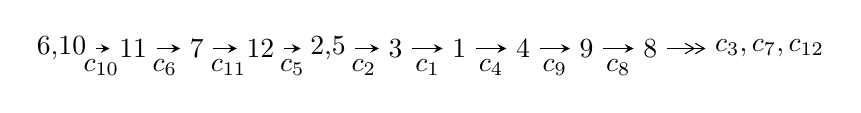
\begin{tikzpicture}[x=23pt, y=7pt]
	% node
	\node (A0) at (-1/8, 0) {6,10};
	\node (A1) at (1, 0) {11};
	\node (A2) at (2, 0) {7};
	\node (A3) at (3, 0) {12};
	\node (A4) at (65/16, 0) {2,5};
	\node (A5) at (41/8, 0) {3};
	\node (A6) at (49/8, 0) {1};
	\node (A7) at (57/8, 0) {4};
	\node (A8) at (65/8, 0) {9};
	\node (A9) at (73/8, 0) {8};
	\node (C1) at (1/2, -1) {$c_{10}$};
	\node (C2) at (3/2, -1) {$c_{6}$};
	\node (C3) at (5/2, -1) {$c_{11}$};
	\node (C4) at (7/2, -1) {$c_{5}$};
	\node (C5) at (37/8, -1) {$c_{2}$};
	\node (C6) at (45/8, -1) {$c_{1}$};
	\node (C7) at (53/8, -1) {$c_{4}$};
	\node (C8) at (61/8, -1) {$c_{9}$};
	\node (C9) at (69/8, -1) {$c_{8}$};
	\node (A10) at (11, 0) {$c_{3},c_{7},c_{12}$};

	% edge
	\draw[->,>=stealth]	
	(A0) edge (A1) (A1) edge (A2) (A2) edge (A3) (A3) edge (A4) (A4) edge (A5) (A5) edge (A6) (A6) edge (A7) (A7) edge (A8) (A8) edge (A9) ;
	\draw[->>,>={angle 60}]	
	(A9) edge (A10);
\end{tikzpicture} \\ 

\end{tabular} \\

\footnotetext{
The image of knot diagram is generated by the software ``\textbf{Draw programme}" developed by Andrew Bartholomew(\url{http://www.layer8.co.uk/maths/draw/index.htm\#Running-draw}), where we modified some parts for our purpose(\url{https://github.com/CATsTAILs/LinksPainter}).
}\phantom \\ \newline 
\centering \textbf{Ideals for irreducible components\footnotemark of $X_{\text{par}}$} 
 
\begin{align*}
I^u_{1}&=\langle 
- u^{20}+10 u^{18}+\cdots+b+2 u,\;u^{23}- u^{22}+\cdots+a-1,\;u^{24}-2 u^{23}+\cdots-8 u^2+1\rangle \\
I^u_{2}&=\langle 
u^4-2 u^2+b+2 u,\;- u^5+3 u^3+a+1,\;u^6+u^5-3 u^4-2 u^3+2 u^2- u-1\rangle \\
\\
\end{align*}
\raggedright * 2 irreducible components of $\dim_{\mathbb{C}}=0$, with total 30 representations.\\
\footnotetext{All coefficients of polynomials are rational numbers. But the coefficients are sometimes approximated in decimal forms when there is not enough margin.}
\newpage
\renewcommand{\arraystretch}{1}
\centering \section*{I. $I^u_{1}= \langle - u^{20}+10 u^{18}+\cdots+b+2 u,\;u^{23}- u^{22}+\cdots+a-1,\;u^{24}-2 u^{23}+\cdots-8 u^2+1 \rangle$}
\flushleft \textbf{(i) Arc colorings}\\
\begin{tabular}{m{7pt} m{180pt} m{7pt} m{180pt} }
\flushright $a_{6}=$&$\begin{pmatrix}0\\u\end{pmatrix}$ \\
\flushright $a_{10}=$&$\begin{pmatrix}1\\0\end{pmatrix}$ \\
\flushright $a_{11}=$&$\begin{pmatrix}1\\u^2\end{pmatrix}$ \\
\flushright $a_{7}=$&$\begin{pmatrix}- u\\- u^3+u\end{pmatrix}$ \\
\flushright $a_{12}=$&$\begin{pmatrix}- u^2+1\\- u^4+2 u^2\end{pmatrix}$ \\
\flushright $a_{2}=$&$\begin{pmatrix}- u^{23}+u^{22}+\cdots+5 u+1\\u^{20}-10 u^{18}+\cdots-6 u^2-2 u\end{pmatrix}$ \\
\flushright $a_{5}=$&$\begin{pmatrix}u\\u\end{pmatrix}$ \\
\flushright $a_{3}=$&$\begin{pmatrix}-2 u^{23}+u^{22}+\cdots+6 u+2\\- u^{23}+12 u^{21}+\cdots- u+1\end{pmatrix}$ \\
\flushright $a_{1}=$&$\begin{pmatrix}u^{10}-5 u^8+8 u^6-5 u^4+3 u^2-1\\u^{12}-6 u^{10}+12 u^8-8 u^6+u^4-2 u^2\end{pmatrix}$ \\
\flushright $a_{4}=$&$\begin{pmatrix}- u^{19}+10 u^{17}+\cdots+5 u+1\\u^{23}- u^{22}+\cdots-2 u-1\end{pmatrix}$ \\
\flushright $a_{9}=$&$\begin{pmatrix}- u^6+3 u^4-2 u^2+1\\- u^8+4 u^6-4 u^4\end{pmatrix}$ \\
\flushright $a_{8}=$&$\begin{pmatrix}- u^{10}+5 u^8-8 u^6+5 u^4-3 u^2+1\\- u^{10}+4 u^8-3 u^6-2 u^4- u^2\end{pmatrix}$\\&\end{tabular}
\flushleft \textbf{(ii) Obstruction class $= -1$}\\~\\
\flushleft \textbf{(iii) Cusp Shapes $= -4 u^{23}+7 u^{22}+45 u^{21}-76 u^{20}-213 u^{19}+331 u^{18}+563 u^{17}-727 u^{16}-961 u^{15}+840 u^{14}+1203 u^{13}-550 u^{12}-1159 u^{11}+373 u^{10}+788 u^9-284 u^8-414 u^7+79 u^6+239 u^5-78 u^4-63 u^3+41 u^2+22 u-6$}\\~\\
\newpage\renewcommand{\arraystretch}{1}
\flushleft \textbf{(iv) u-Polynomials at the component}\newline \\
\begin{tabular}{m{50pt}|m{274pt}}
Crossings & \hspace{64pt}u-Polynomials at each crossing \\
\hline $$\begin{aligned}c_{1}\end{aligned}$$&$\begin{aligned}
&u^{24}+u^{23}+\cdots+33 u+1
\end{aligned}$\\
\hline $$\begin{aligned}c_{2},c_{4}\end{aligned}$$&$\begin{aligned}
&u^{24}-7 u^{23}+\cdots-9 u+1
\end{aligned}$\\
\hline $$\begin{aligned}c_{3},c_{7}\end{aligned}$$&$\begin{aligned}
&u^{24}- u^{23}+\cdots+64 u+64
\end{aligned}$\\
\hline $$\begin{aligned}c_{5},c_{6},c_{10}\\c_{11}\end{aligned}$$&$\begin{aligned}
&u^{24}-2 u^{23}+\cdots-8 u^2+1
\end{aligned}$\\
\hline $$\begin{aligned}c_{8}\end{aligned}$$&$\begin{aligned}
&u^{24}+2 u^{23}+\cdots+7956 u+4721
\end{aligned}$\\
\hline $$\begin{aligned}c_{9},c_{12}\end{aligned}$$&$\begin{aligned}
&u^{24}-2 u^{23}+\cdots+2 u+1
\end{aligned}$\\
\hline
\end{tabular}\\~\\
\newpage\renewcommand{\arraystretch}{1}
\flushleft \textbf{(v) Riley Polynomials at the component}\newline \\
\begin{tabular}{m{50pt}|m{274pt}}
Crossings & \hspace{64pt}Riley Polynomials at each crossing \\
\hline $$\begin{aligned}c_{1}\end{aligned}$$&$\begin{aligned}
&y^{24}+51 y^{23}+\cdots-789 y+1
\end{aligned}$\\
\hline $$\begin{aligned}c_{2},c_{4}\end{aligned}$$&$\begin{aligned}
&y^{24}- y^{23}+\cdots-33 y+1
\end{aligned}$\\
\hline $$\begin{aligned}c_{3},c_{7}\end{aligned}$$&$\begin{aligned}
&y^{24}-39 y^{23}+\cdots-65536 y+4096
\end{aligned}$\\
\hline $$\begin{aligned}c_{5},c_{6},c_{10}\\c_{11}\end{aligned}$$&$\begin{aligned}
&y^{24}-26 y^{23}+\cdots-16 y+1
\end{aligned}$\\
\hline $$\begin{aligned}c_{8}\end{aligned}$$&$\begin{aligned}
&y^{24}+94 y^{23}+\cdots-805269180 y+22287841
\end{aligned}$\\
\hline $$\begin{aligned}c_{9},c_{12}\end{aligned}$$&$\begin{aligned}
&y^{24}+34 y^{23}+\cdots-16 y+1
\end{aligned}$\\
\hline
\end{tabular}\\~\\
\newpage\flushleft \textbf{(vi) Complex Volumes and Cusp Shapes}
$$\begin{array}{c|c|c}  
\text{Solutions to }I^u_{1}& \I (\text{vol} + \sqrt{-1}CS) & \text{Cusp shape}\\
 \hline 
\begin{aligned}
u &= -0.546136 + 0.704998 I \\
a &= \phantom{-}0.218919 + 0.545111 I \\
b &= -1.58637 + 0.30753 I\end{aligned}
 & \phantom{-}13.8157 + 6.6372 I & -5.51662 - 4.82221 I \\ \hline\begin{aligned}
u &= -0.546136 - 0.704998 I \\
a &= \phantom{-}0.218919 - 0.545111 I \\
b &= -1.58637 - 0.30753 I\end{aligned}
 & \phantom{-}13.8157 - 6.6372 I & -5.51662 + 4.82221 I \\ \hline\begin{aligned}
u &= -0.490937 + 0.721217 I \\
a &= -0.42824 + 1.49833 I \\
b &= -0.020820 - 0.317218 I\end{aligned}
 & \phantom{-}13.98230 - 1.87133 I & -5.11127 - 0.61495 I \\ \hline\begin{aligned}
u &= -0.490937 - 0.721217 I \\
a &= -0.42824 - 1.49833 I \\
b &= -0.020820 + 0.317218 I\end{aligned}
 & \phantom{-}13.98230 + 1.87133 I & -5.11127 + 0.61495 I \\ \hline\begin{aligned}
u &= \phantom{-}0.581256 + 0.532393 I \\
a &= \phantom{-}0.124238 + 0.261688 I \\
b &= \phantom{-}1.180950 + 0.505513 I\end{aligned}
 & \phantom{-}2.81700 - 3.48253 I & -5.09473 + 5.87430 I \\ \hline\begin{aligned}
u &= \phantom{-}0.581256 - 0.532393 I \\
a &= \phantom{-}0.124238 - 0.261688 I \\
b &= \phantom{-}1.180950 - 0.505513 I\end{aligned}
 & \phantom{-}2.81700 + 3.48253 I & -5.09473 - 5.87430 I \\ \hline\begin{aligned}
u &= \phantom{-}0.371044 + 0.593072 I \\
a &= \phantom{-}0.614735 + 1.078340 I \\
b &= -0.138383 + 0.111177 I\end{aligned}
 & \phantom{-}3.46440 - 0.36969 I & -3.22680 + 1.74990 I \\ \hline\begin{aligned}
u &= \phantom{-}0.371044 - 0.593072 I \\
a &= \phantom{-}0.614735 - 1.078340 I \\
b &= -0.138383 - 0.111177 I\end{aligned}
 & \phantom{-}3.46440 + 0.36969 I & -3.22680 - 1.74990 I \\ \hline\begin{aligned}
u &= -0.560055\phantom{ +0.000000I} \\
a &= -0.358547\phantom{ +0.000000I} \\
b &= -0.698358\phantom{ +0.000000I}\end{aligned}
 & -0.920303\phantom{ +0.000000I} & -10.4000\phantom{ +0.000000I} \\ \hline\begin{aligned}
u &= -1.44707 + 0.16024 I \\
a &= -0.1025080 + 0.0199673 I \\
b &= -0.075688 - 0.613179 I\end{aligned}
 & -2.38092 + 3.00213 I & -7.53165 - 2.42924 I\\
 \hline 
 \end{array}$$\newpage$$\begin{array}{c|c|c}  
\text{Solutions to }I^u_{1}& \I (\text{vol} + \sqrt{-1}CS) & \text{Cusp shape}\\
 \hline 
\begin{aligned}
u &= -1.44707 - 0.16024 I \\
a &= -0.1025080 - 0.0199673 I \\
b &= -0.075688 + 0.613179 I\end{aligned}
 & -2.38092 - 3.00213 I & -7.53165 + 2.42924 I \\ \hline\begin{aligned}
u &= \phantom{-}1.46661 + 0.06456 I \\
a &= -1.18298 + 1.35435 I \\
b &= -1.81615 + 1.04191 I\end{aligned}
 & -6.76285 - 2.21001 I & -11.76840 + 2.54579 I \\ \hline\begin{aligned}
u &= \phantom{-}1.46661 - 0.06456 I \\
a &= -1.18298 - 1.35435 I \\
b &= -1.81615 - 1.04191 I\end{aligned}
 & -6.76285 + 2.21001 I & -11.76840 - 2.54579 I \\ \hline\begin{aligned}
u &= -1.47571\phantom{ +0.000000I} \\
a &= \phantom{-}3.35878\phantom{ +0.000000I} \\
b &= \phantom{-}4.21798\phantom{ +0.000000I}\end{aligned}
 & -8.10337\phantom{ +0.000000I} & -9.82550\phantom{ +0.000000I} \\ \hline\begin{aligned}
u &= \phantom{-}1.50201 + 0.24602 I \\
a &= \phantom{-}0.543477 - 0.750165 I \\
b &= \phantom{-}1.09231 - 1.65332 I\end{aligned}
 & \phantom{-}7.50585 - 1.64558 I & -8.27015 + 0.73963 I \\ \hline\begin{aligned}
u &= \phantom{-}1.50201 - 0.24602 I \\
a &= \phantom{-}0.543477 + 0.750165 I \\
b &= \phantom{-}1.09231 + 1.65332 I\end{aligned}
 & \phantom{-}7.50585 + 1.64558 I & -8.27015 - 0.73963 I \\ \hline\begin{aligned}
u &= -0.344587 + 0.302443 I \\
a &= -1.119750 + 0.097114 I \\
b &= \phantom{-}0.366639 + 0.663744 I\end{aligned}
 & -0.814955 + 1.024630 I & -8.91038 - 6.27818 I \\ \hline\begin{aligned}
u &= -0.344587 - 0.302443 I \\
a &= -1.119750 - 0.097114 I \\
b &= \phantom{-}0.366639 - 0.663744 I\end{aligned}
 & -0.814955 - 1.024630 I & -8.91038 + 6.27818 I \\ \hline\begin{aligned}
u &= \phantom{-}1.53592 + 0.23426 I \\
a &= \phantom{-}2.64852 - 0.49160 I \\
b &= \phantom{-}3.50928 + 0.08824 I\end{aligned}
 & \phantom{-}6.98523 - 10.07590 I & -8.82304 + 4.75008 I \\ \hline\begin{aligned}
u &= \phantom{-}1.53592 - 0.23426 I \\
a &= \phantom{-}2.64852 + 0.49160 I \\
b &= \phantom{-}3.50928 - 0.08824 I\end{aligned}
 & \phantom{-}6.98523 + 10.07590 I & -8.82304 - 4.75008 I\\
 \hline 
 \end{array}$$\newpage$$\begin{array}{c|c|c}  
\text{Solutions to }I^u_{1}& \I (\text{vol} + \sqrt{-1}CS) & \text{Cusp shape}\\
 \hline 
\begin{aligned}
u &= \phantom{-}1.55778\phantom{ +0.000000I} \\
a &= \phantom{-}2.20275\phantom{ +0.000000I} \\
b &= \phantom{-}2.47794\phantom{ +0.000000I}\end{aligned}
 & -8.18010\phantom{ +0.000000I} & -9.41090\phantom{ +0.000000I} \\ \hline\begin{aligned}
u &= -1.55100 + 0.14681 I \\
a &= -2.45672 - 0.03517 I \\
b &= -2.88742 + 0.30740 I\end{aligned}
 & -4.30018 + 5.91154 I & -8.53274 - 5.50143 I \\ \hline\begin{aligned}
u &= -1.55100 - 0.14681 I \\
a &= -2.45672 + 0.03517 I \\
b &= -2.88742 - 0.30740 I\end{aligned}
 & -4.30018 - 5.91154 I & -8.53274 + 5.50143 I \\ \hline\begin{aligned}
u &= \phantom{-}0.323756\phantom{ +0.000000I} \\
a &= \phantom{-}2.07762\phantom{ +0.000000I} \\
b &= -1.24627\phantom{ +0.000000I}\end{aligned}
 & -2.07138\phantom{ +0.000000I} & \phantom{-}3.20840\phantom{ +0.000000I}\\
 \hline 
 \end{array}$$\newpage\newpage\renewcommand{\arraystretch}{1}
\centering \section*{II. $I^u_{2}= \langle u^4-2 u^2+b+2 u,\;- u^5+3 u^3+a+1,\;u^6+u^5-3 u^4-2 u^3+2 u^2- u-1 \rangle$}
\flushleft \textbf{(i) Arc colorings}\\
\begin{tabular}{m{7pt} m{180pt} m{7pt} m{180pt} }
\flushright $a_{6}=$&$\begin{pmatrix}0\\u\end{pmatrix}$ \\
\flushright $a_{10}=$&$\begin{pmatrix}1\\0\end{pmatrix}$ \\
\flushright $a_{11}=$&$\begin{pmatrix}1\\u^2\end{pmatrix}$ \\
\flushright $a_{7}=$&$\begin{pmatrix}- u\\- u^3+u\end{pmatrix}$ \\
\flushright $a_{12}=$&$\begin{pmatrix}- u^2+1\\- u^4+2 u^2\end{pmatrix}$ \\
\flushright $a_{2}=$&$\begin{pmatrix}u^5-3 u^3-1\\- u^4+2 u^2-2 u\end{pmatrix}$ \\
\flushright $a_{5}=$&$\begin{pmatrix}u\\u\end{pmatrix}$ \\
\flushright $a_{3}=$&$\begin{pmatrix}u^5-3 u^3+u-1\\- u^4+2 u^2- u\end{pmatrix}$ \\
\flushright $a_{1}=$&$\begin{pmatrix}- u\\- u\end{pmatrix}$ \\
\flushright $a_{4}=$&$\begin{pmatrix}u^5-3 u^3+u-1\\- u^4+2 u^2- u\end{pmatrix}$ \\
\flushright $a_{9}=$&$\begin{pmatrix}u^5-2 u^3- u\\u^5-3 u^3+u\end{pmatrix}$ \\
\flushright $a_{8}=$&$\begin{pmatrix}- u\\- u^3+u\end{pmatrix}$\\&\end{tabular}
\flushleft \textbf{(ii) Obstruction class $= 1$}\\~\\
\flushleft \textbf{(iii) Cusp Shapes $= 3 u^5+u^4-14 u^3- u^2+14 u-18$}\\~\\
\newpage\renewcommand{\arraystretch}{1}
\flushleft \textbf{(iv) u-Polynomials at the component}\newline \\
\begin{tabular}{m{50pt}|m{274pt}}
Crossings & \hspace{64pt}u-Polynomials at each crossing \\
\hline $$\begin{aligned}c_{1},c_{2}\end{aligned}$$&$\begin{aligned}
&(u-1)^6
\end{aligned}$\\
\hline $$\begin{aligned}c_{3},c_{7}\end{aligned}$$&$\begin{aligned}
&u^6
\end{aligned}$\\
\hline $$\begin{aligned}c_{4}\end{aligned}$$&$\begin{aligned}
&(u+1)^6
\end{aligned}$\\
\hline $$\begin{aligned}c_{5},c_{6}\end{aligned}$$&$\begin{aligned}
&u^6- u^5-3 u^4+2 u^3+2 u^2+u-1
\end{aligned}$\\
\hline $$\begin{aligned}c_{8},c_{12}\end{aligned}$$&$\begin{aligned}
&u^6- u^5+3 u^4-2 u^3+2 u^2- u-1
\end{aligned}$\\
\hline $$\begin{aligned}c_{9}\end{aligned}$$&$\begin{aligned}
&u^6+u^5+3 u^4+2 u^3+2 u^2+u-1
\end{aligned}$\\
\hline $$\begin{aligned}c_{10},c_{11}\end{aligned}$$&$\begin{aligned}
&u^6+u^5-3 u^4-2 u^3+2 u^2- u-1
\end{aligned}$\\
\hline
\end{tabular}\\~\\
\newpage\renewcommand{\arraystretch}{1}
\flushleft \textbf{(v) Riley Polynomials at the component}\newline \\
\begin{tabular}{m{50pt}|m{274pt}}
Crossings & \hspace{64pt}Riley Polynomials at each crossing \\
\hline $$\begin{aligned}c_{1},c_{2},c_{4}\end{aligned}$$&$\begin{aligned}
&(y-1)^6
\end{aligned}$\\
\hline $$\begin{aligned}c_{3},c_{7}\end{aligned}$$&$\begin{aligned}
&y^6
\end{aligned}$\\
\hline $$\begin{aligned}c_{5},c_{6},c_{10}\\c_{11}\end{aligned}$$&$\begin{aligned}
&y^6-7 y^5+17 y^4-16 y^3+6 y^2-5 y+1
\end{aligned}$\\
\hline $$\begin{aligned}c_{8},c_{9},c_{12}\end{aligned}$$&$\begin{aligned}
&y^6+5 y^5+9 y^4+4 y^3-6 y^2-5 y+1
\end{aligned}$\\
\hline
\end{tabular}\\~\\
\newpage\flushleft \textbf{(vi) Complex Volumes and Cusp Shapes}
$$\begin{array}{c|c|c}  
\text{Solutions to }I^u_{2}& \I (\text{vol} + \sqrt{-1}CS) & \text{Cusp shape}\\
 \hline 
\begin{aligned}
u &= \phantom{-}0.493180 + 0.575288 I \\
a &= \phantom{-}0.011399 - 0.918055 I \\
b &= -0.847526 + 0.083869 I\end{aligned}
 & \phantom{-}1.31531 - 1.97241 I & -6.43930 + 3.48596 I \\ \hline\begin{aligned}
u &= \phantom{-}0.493180 - 0.575288 I \\
a &= \phantom{-}0.011399 + 0.918055 I \\
b &= -0.847526 - 0.083869 I\end{aligned}
 & \phantom{-}1.31531 + 1.97241 I & -6.43930 - 3.48596 I \\ \hline\begin{aligned}
u &= -0.483672\phantom{ +0.000000I} \\
a &= -0.687021\phantom{ +0.000000I} \\
b &= \phantom{-}1.38049\phantom{ +0.000000I}\end{aligned}
 & -2.38379\phantom{ +0.000000I} & -23.4460\phantom{ +0.000000I} \\ \hline\begin{aligned}
u &= -1.52087 + 0.16310 I \\
a &= \phantom{-}1.98288 + 0.88048 I \\
b &= \phantom{-}2.63293 + 0.95019 I\end{aligned}
 & -5.34051 + 4.59213 I & -10.66600 - 2.48468 I \\ \hline\begin{aligned}
u &= -1.52087 - 0.16310 I \\
a &= \phantom{-}1.98288 - 0.88048 I \\
b &= \phantom{-}2.63293 - 0.95019 I\end{aligned}
 & -5.34051 - 4.59213 I & -10.66600 + 2.48468 I \\ \hline\begin{aligned}
u &= \phantom{-}1.53904\phantom{ +0.000000I} \\
a &= -3.30155\phantom{ +0.000000I} \\
b &= -3.95130\phantom{ +0.000000I}\end{aligned}
 & -9.30502\phantom{ +0.000000I} & -18.3430\phantom{ +0.000000I}\\
 \hline 
 \end{array}$$\newpage
\newpage\renewcommand{\arraystretch}{1}
\centering \section*{ III. u-Polynomials}
\begin{tabular}{m{50pt}|m{274pt}}
Crossings & \hspace{64pt}u-Polynomials at each crossing \\
\hline $$\begin{aligned}c_{1}\end{aligned}$$&$\begin{aligned}
&((u-1)^6)(u^{24}+u^{23}+\cdots+33 u+1)
\end{aligned}$\\
\hline $$\begin{aligned}c_{2}\end{aligned}$$&$\begin{aligned}
&((u-1)^6)(u^{24}-7 u^{23}+\cdots-9 u+1)
\end{aligned}$\\
\hline $$\begin{aligned}c_{3},c_{7}\end{aligned}$$&$\begin{aligned}
&u^6(u^{24}- u^{23}+\cdots+64 u+64)
\end{aligned}$\\
\hline $$\begin{aligned}c_{4}\end{aligned}$$&$\begin{aligned}
&((u+1)^6)(u^{24}-7 u^{23}+\cdots-9 u+1)
\end{aligned}$\\
\hline $$\begin{aligned}c_{5},c_{6}\end{aligned}$$&$\begin{aligned}
&(u^6- u^5-3 u^4+2 u^3+2 u^2+u-1)(u^{24}-2 u^{23}+\cdots-8 u^2+1)
\end{aligned}$\\
\hline $$\begin{aligned}c_{8}\end{aligned}$$&$\begin{aligned}
&(u^6- u^5+3 u^4-2 u^3+2 u^2- u-1)(u^{24}+2 u^{23}+\cdots+7956 u+4721)
\end{aligned}$\\
\hline $$\begin{aligned}c_{9}\end{aligned}$$&$\begin{aligned}
&(u^6+u^5+3 u^4+2 u^3+2 u^2+u-1)(u^{24}-2 u^{23}+\cdots+2 u+1)
\end{aligned}$\\
\hline $$\begin{aligned}c_{10},c_{11}\end{aligned}$$&$\begin{aligned}
&(u^6+u^5-3 u^4-2 u^3+2 u^2- u-1)(u^{24}-2 u^{23}+\cdots-8 u^2+1)
\end{aligned}$\\
\hline $$\begin{aligned}c_{12}\end{aligned}$$&$\begin{aligned}
&(u^6- u^5+3 u^4-2 u^3+2 u^2- u-1)(u^{24}-2 u^{23}+\cdots+2 u+1)
\end{aligned}$\\
\hline
\end{tabular}\newpage\renewcommand{\arraystretch}{1}
\centering \section*{ IV. Riley Polynomials}
\begin{tabular}{m{50pt}|m{274pt}}
Crossings & \hspace{64pt}Riley Polynomials at each crossing \\
\hline $$\begin{aligned}c_{1}\end{aligned}$$&$\begin{aligned}
&((y-1)^6)(y^{24}+51 y^{23}+\cdots-789 y+1)
\end{aligned}$\\
\hline $$\begin{aligned}c_{2},c_{4}\end{aligned}$$&$\begin{aligned}
&((y-1)^6)(y^{24}- y^{23}+\cdots-33 y+1)
\end{aligned}$\\
\hline $$\begin{aligned}c_{3},c_{7}\end{aligned}$$&$\begin{aligned}
&y^6(y^{24}-39 y^{23}+\cdots-65536 y+4096)
\end{aligned}$\\
\hline $$\begin{aligned}c_{5},c_{6},c_{10}\\c_{11}\end{aligned}$$&$\begin{aligned}
&(y^6-7 y^5+\cdots-5 y+1)(y^{24}-26 y^{23}+\cdots-16 y+1)
\end{aligned}$\\
\hline $$\begin{aligned}c_{8}\end{aligned}$$&$\begin{aligned}
&(y^6+5 y^5+9 y^4+4 y^3-6 y^2-5 y+1)\\
&\cdot(y^{24}+94 y^{23}+\cdots-805269180 y+22287841)
\end{aligned}$\\
\hline $$\begin{aligned}c_{9},c_{12}\end{aligned}$$&$\begin{aligned}
&(y^6+5 y^5+\cdots-5 y+1)(y^{24}+34 y^{23}+\cdots-16 y+1)
\end{aligned}$\\
\hline
\end{tabular}
\vskip 2pc
\end{document}